\documentclass[border=10pt]{standalone}
\usepackage{tikz}\usepackage{amsmath}\usetikzlibrary{arrows.meta,positioning}
\begin{document}
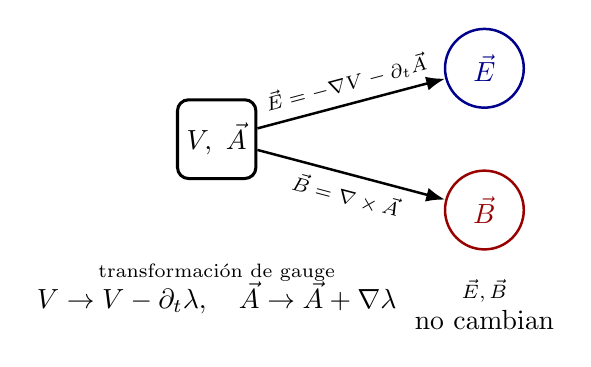
\begin{tikzpicture}[line width=0.9pt,>={Latex[length=2.4mm]}]
  \node[draw,rounded corners,line width=1.1pt,minimum height=1cm] (pot) at (0,0){$V,\ \vec A$};
  \node[draw,circle,blue!55!black,minimum size=1cm] (E) at (3.4,0.9){$\vec E$};
  \node[draw,circle,red!60!black,minimum size=1cm] (B) at (3.4,-0.9){$\vec B$};
  \draw[->] (pot) to node[above,sloped]{\scriptsize $\vec E=-\nabla V-\partial_t\vec A$} (E);
  \draw[->] (pot) to node[below,sloped]{\scriptsize $\vec B=\nabla\times\vec A$} (B);
  \node[align=center] at (0,-1.9){\scriptsize transformación de gauge\\[-1pt]$V\to V-\partial_t\lambda,\quad \vec A\to\vec A+\nabla\lambda$};
  \node[align=center] at (3.4,-2.1){\scriptsize $\vec E,\vec B$ \\[-1pt]no cambian};
\end{tikzpicture}
\end{document}
